
\documentclass{article}

% ---------------------------------------------------------------------------
% ICLR 2027 workshop version (short). The full version is main.tex; every
% number here is quoted from it. Anonymized for double-blind review.
% Compile:  pdflatex workshop && bibtex workshop && pdflatex workshop x2
% ---------------------------------------------------------------------------

\usepackage{iclr2027_conference,times}
\usepackage{amsmath,amssymb,amsthm}
\usepackage{graphicx}
\usepackage{booktabs}
\usepackage{caption}
\usepackage{xcolor}
\usepackage[colorlinks=true,linkcolor=blue,citecolor=blue,urlcolor=blue]{hyperref}
\usepackage{enumitem}

\graphicspath{{figures/}}

\theoremstyle{plain}
\newtheorem{proposition}{Proposition}
\newtheorem{theorem}{Theorem}
\newtheorem{lemma}{Lemma}
\newtheorem{corollary}{Corollary}
\theoremstyle{remark}
\newtheorem{remark}{Remark}

%%%%% MATH DEFINITIONS, shared by the body and Appendix A %%%%%
% Read by main.tex with %%%%% MATH DEFINITIONS, shared by the body and Appendix A %%%%%
% Read by main.tex with %%%%% MATH DEFINITIONS, shared by the body and Appendix A %%%%%
% Read by main.tex with \input{math_commands}. Proofs use the shorthands at the end,
% so that a display is a line of mathematics and not a line of \frac's.

% --- sets and operators ---------------------------------------------------
\newcommand{\R}{\mathbb{R}}
\newcommand{\E}{\mathbb{E}}
\newcommand{\Var}{\operatorname{Var}}
\newcommand{\Cov}{\operatorname{Cov}}
\newcommand{\tr}{\operatorname{tr}}
\newcommand{\N}{\mathcal{N}}
\newcommand{\D}{\mathcal{D}}
\newcommand{\dist}{\operatorname{dist}}
\newcommand{\supp}{\operatorname{supp}}
\newcommand{\law}{\mathrm{Law}}
\newcommand{\ind}{\mathbf{1}}
\newcommand{\eps}{\varepsilon}

% --- objects of the paper -------------------------------------------------
\newcommand{\Sigmapost}{\Sigma_{\mathrm{post}}}
\newcommand{\Xhat}{\widehat{\Sigma}_X}
\newcommand{\rhohat}{\widehat{\rho}}
\newcommand{\vstar}{v_h^\star}
\newcommand{\vstarz}{v_0^\star}
\newcommand{\Covh}{\operatorname{Cov}_h}

% --- shorthands for the proofs --------------------------------------------
% label weight and kernel weight of atom #1 at bandwidth h
\newcommand{\pih}[1]{p_{#1}^{(h)}}
\newcommand{\wih}[1]{w_{#1}^{(h)}}
% label kernel K_h(y - y^i)
\newcommand{\KK}[1]{K_h(y-y^{#1})}
% per-atom collapsed field (x^i - x)/(1 - t)
\newcommand{\fat}[1]{\frac{x^{#1}-x}{1-t}}
% source density at the point that reaches x from atom #1
\newcommand{\src}[1]{\pi_0\!\Big(\frac{x-tx^{#1}}{1-t}\Big)}

% --- pointer from a statement in the body to its proof --------------------
\newcommand{\proofin}[1]{\hfill\textnormal{\footnotesize[Proof: Appendix~\ref{#1}]}}
. Proofs use the shorthands at the end,
% so that a display is a line of mathematics and not a line of \frac's.

% --- sets and operators ---------------------------------------------------
\newcommand{\R}{\mathbb{R}}
\newcommand{\E}{\mathbb{E}}
\newcommand{\Var}{\operatorname{Var}}
\newcommand{\Cov}{\operatorname{Cov}}
\newcommand{\tr}{\operatorname{tr}}
\newcommand{\N}{\mathcal{N}}
\newcommand{\D}{\mathcal{D}}
\newcommand{\dist}{\operatorname{dist}}
\newcommand{\supp}{\operatorname{supp}}
\newcommand{\law}{\mathrm{Law}}
\newcommand{\ind}{\mathbf{1}}
\newcommand{\eps}{\varepsilon}

% --- objects of the paper -------------------------------------------------
\newcommand{\Sigmapost}{\Sigma_{\mathrm{post}}}
\newcommand{\Xhat}{\widehat{\Sigma}_X}
\newcommand{\rhohat}{\widehat{\rho}}
\newcommand{\vstar}{v_h^\star}
\newcommand{\vstarz}{v_0^\star}
\newcommand{\Covh}{\operatorname{Cov}_h}

% --- shorthands for the proofs --------------------------------------------
% label weight and kernel weight of atom #1 at bandwidth h
\newcommand{\pih}[1]{p_{#1}^{(h)}}
\newcommand{\wih}[1]{w_{#1}^{(h)}}
% label kernel K_h(y - y^i)
\newcommand{\KK}[1]{K_h(y-y^{#1})}
% per-atom collapsed field (x^i - x)/(1 - t)
\newcommand{\fat}[1]{\frac{x^{#1}-x}{1-t}}
% source density at the point that reaches x from atom #1
\newcommand{\src}[1]{\pi_0\!\Big(\frac{x-tx^{#1}}{1-t}\Big)}

% --- pointer from a statement in the body to its proof --------------------
\newcommand{\proofin}[1]{\hfill\textnormal{\footnotesize[Proof: Appendix~\ref{#1}]}}
. Proofs use the shorthands at the end,
% so that a display is a line of mathematics and not a line of \frac's.

% --- sets and operators ---------------------------------------------------
\newcommand{\R}{\mathbb{R}}
\newcommand{\E}{\mathbb{E}}
\newcommand{\Var}{\operatorname{Var}}
\newcommand{\Cov}{\operatorname{Cov}}
\newcommand{\tr}{\operatorname{tr}}
\newcommand{\N}{\mathcal{N}}
\newcommand{\D}{\mathcal{D}}
\newcommand{\dist}{\operatorname{dist}}
\newcommand{\supp}{\operatorname{supp}}
\newcommand{\law}{\mathrm{Law}}
\newcommand{\ind}{\mathbf{1}}
\newcommand{\eps}{\varepsilon}

% --- objects of the paper -------------------------------------------------
\newcommand{\Sigmapost}{\Sigma_{\mathrm{post}}}
\newcommand{\Xhat}{\widehat{\Sigma}_X}
\newcommand{\rhohat}{\widehat{\rho}}
\newcommand{\vstar}{v_h^\star}
\newcommand{\vstarz}{v_0^\star}
\newcommand{\Covh}{\operatorname{Cov}_h}

% --- shorthands for the proofs --------------------------------------------
% label weight and kernel weight of atom #1 at bandwidth h
\newcommand{\pih}[1]{p_{#1}^{(h)}}
\newcommand{\wih}[1]{w_{#1}^{(h)}}
% label kernel K_h(y - y^i)
\newcommand{\KK}[1]{K_h(y-y^{#1})}
% per-atom collapsed field (x^i - x)/(1 - t)
\newcommand{\fat}[1]{\frac{x^{#1}-x}{1-t}}
% source density at the point that reaches x from atom #1
\newcommand{\src}[1]{\pi_0\!\Big(\frac{x-tx^{#1}}{1-t}\Big)}

% --- pointer from a statement in the body to its proof --------------------
\newcommand{\proofin}[1]{\hfill\textnormal{\footnotesize[Proof: Appendix~\ref{#1}]}}


\title{Trained Conditional Flows Memorise\\
at an Effective Bandwidth}

\author{Anonymous authors \\ Paper under double-blind review}

\begin{document}
\maketitle

\begin{abstract}
A conditional flow trained on finite data behaves like Nadaraya--Watson regression over
its training examples at a single effective bandwidth $h_{\mathrm{eff}}$, which
training shrinks towards the bandwidth $h$ of the label noise it was given. The
reference comes from exact theory: with the training set fixed, the population
minimiser sends a condition that identifies one example to that example, and label
smoothing at bandwidth $h$ turns its endpoint law into a Nadaraya--Watson mixture of the
training atoms, atomic at every $h$. Fitting that reference to a trained model's
per-condition variances gives $h_{\mathrm{eff}}$; fitting it to the per-condition means,
separately, gives the same bandwidth within 95\% intervals at $48/48$ checkpoints of 15
synthetic runs and $31/36$ of six CIFAR-10 runs with a $35.75$M-parameter U-Net. In
both, $h_{\mathrm{eff}}$ falls monotonically with training and ends at $1.08h$
(synthetic) and $1.13$--$1.34h$ (CIFAR-10, $60$k iterations). Where the posterior is
known, $h_{\mathrm{eff}}$ read from the training conditions ranks the coverage of
posterior credible regions at held-out conditions with Spearman $0.90$, and the sampler
stays calibrated while $h_{\mathrm{eff}}$ stays in a window. The account turns the
memorisation of a conditional sampler into one number that can be read off a
checkpoint.
\end{abstract}

% ==========================================================================
\section{Introduction}

Flow matching \citep{lipman2023flow,albergo2023building,liu2023rectified} regresses a
velocity field on a path from noise to data. Used for posterior sampling in inverse
problems, conditional flow matching is calibrated early in training and then becomes
nearly deterministic, returning training examples \citep{physicscfm2026}. That the
empirical minimiser memorises is known in the unconditional case
\citep{gao2024flow,bertrand2025closed,kamb2024creativity,buchanan2025edge,li2026memory}.
We ask what the conditional minimiser does, and what a practitioner's usual fix,
Gaussian noise on the condition \citep{ho2022cascaded,sadat2024cads}, actually buys.

This is an analysis of model behaviour, built on exact theory. With the training set
fixed:
\begin{itemize}[leftmargin=1.4em,itemsep=1pt,topsep=2pt]
\item a condition that identifies its example gives an endpoint law $\delta_{x^i}$ with
  zero variance and zero loss (Proposition~\ref{prop:collapse});
\item label smoothing at bandwidth $h$ gives the Nadaraya--Watson mixture
  $\sum_ip_i^{(h)}(y)\delta_{x^i}$ (Theorem~\ref{thm:endpoint}), atomic at every $h$
  with a Wasserstein floor independent of $h$ (Proposition~\ref{prop:atomicity});
\item \textbf{a trained model follows that mixture at one effective bandwidth}
  $h_{\mathrm{eff}}$, shared by all conditions and identified independently by the
  generated variances and the generated means; $h_{\mathrm{eff}}$ falls towards $h$
  as training proceeds (Section~\ref{sec:heff}).
\end{itemize}
The first two results are the population optimum; the third says how far a finite
network has gone towards it, and makes memorisation a single number read off a
checkpoint (Section~\ref{sec:audit}).
\citet{smola2026support} read the spatial factor of the same index posterior as a kernel
smoother in time; we use the label factor, whose bandwidth is a modelling choice and
survives to $t=1$.

\begin{figure}[t]
\centering
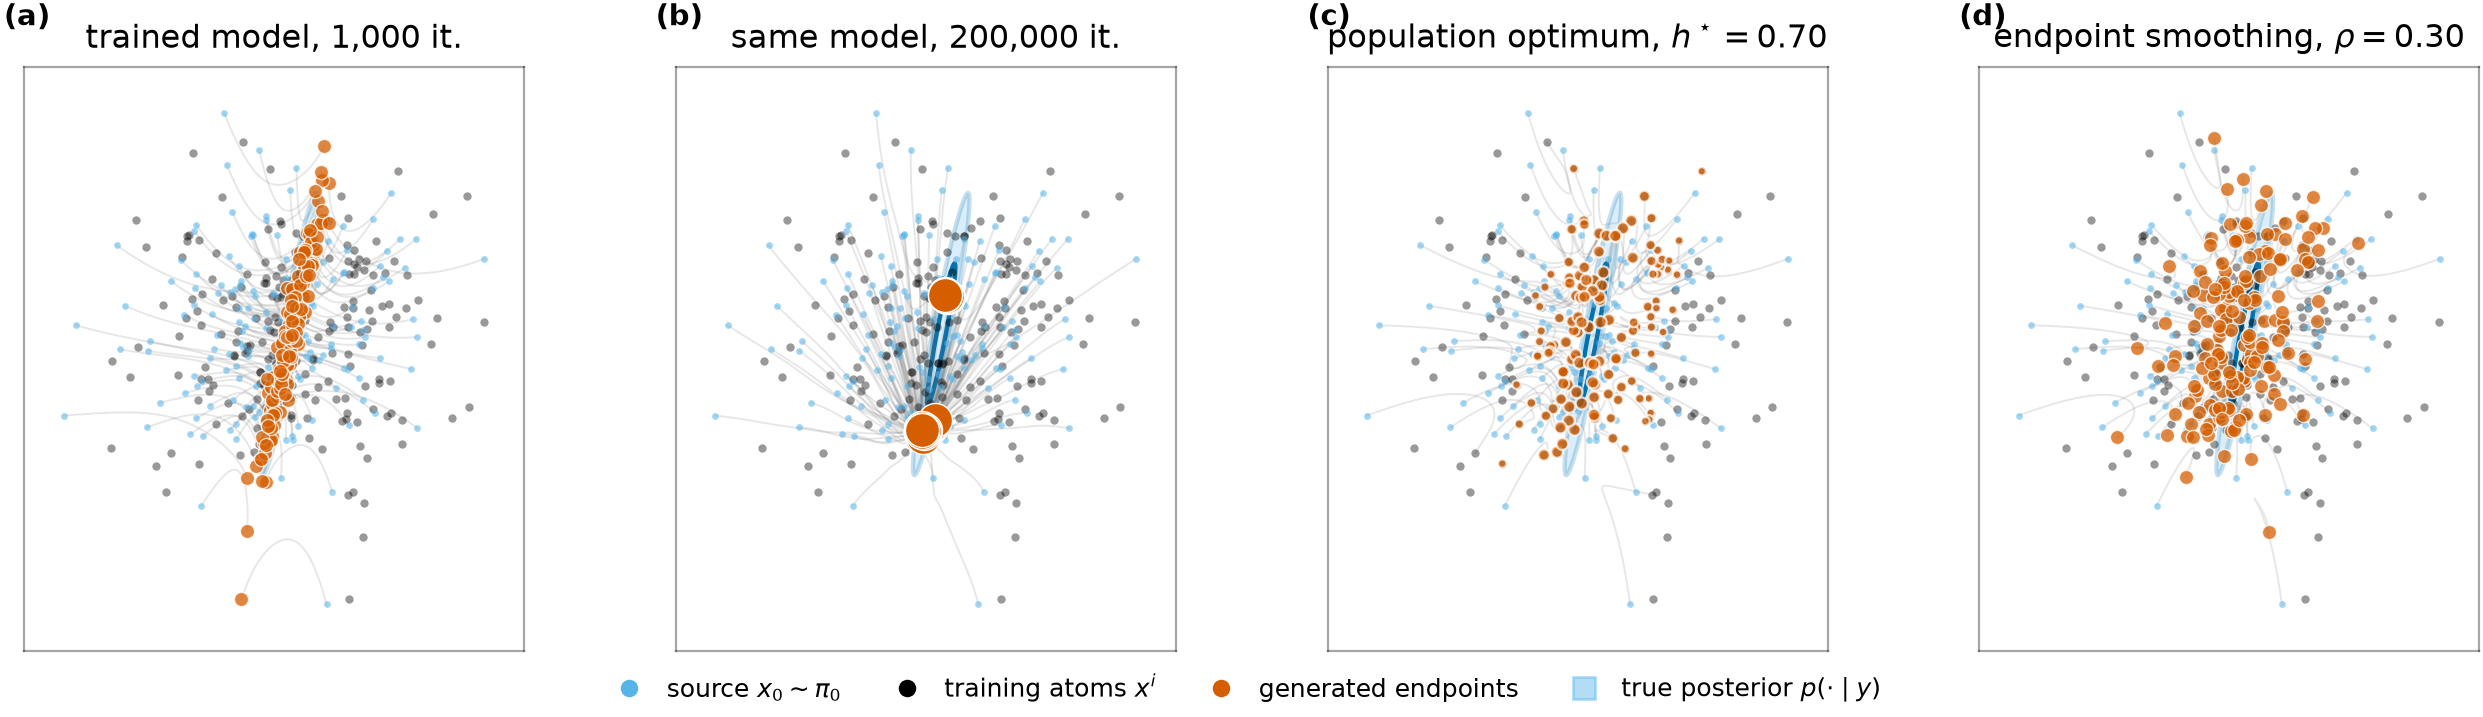
\includegraphics[width=\textwidth]{fig_flow_portrait.png}
\caption{One condition of the synthetic instance ($d{=}2$, $N{=}200$), $160$ source
draws. (a,~b) A trained network at $10^3$ and $2\times10^5$ iterations: first a
posterior sampler, then $96\%$ of paths end on the labelled atom. (c) The population
optimum at the bandwidth whose $\tr\Covh$ equals $\tr\Sigmapost$; marker area is
$p_i^{(h)}$. The variance is right and the law is still atomic. (d) Endpoint noise
leaves the atoms.}
\label{fig:mechanism}
\end{figure}

% ==========================================================================
\section{Exact population theory}
\label{sec:theory}

Fix $\D=\{(x^i,y^i)\}_{i=1}^N$ with $x^i\in\R^d$, $y^i\in\R^k$ and $y^i\ne y^j$ for
$i\ne j$; identifying conditions of this kind are the norm in inverse problems and
inpainting. Draw $I\sim\mathrm{Unif}\{1,\dots,N\}$, $X_0\sim\pi_0=\N(0,I_d)$,
$t\sim\mathrm{Unif}(0,1)$, $\eps\sim\N(0,I_k)$, and set $X_t=(1-t)X_0+tx^I$,
$U=x^I-X_0$, $\widetilde Y=y^I+h\eps$. The objective is
$L_h(v)=\E|U-v(X_t,t,\widetilde Y)|^2$ over square-integrable $v$; its minimiser is
$\vstar=\E[U\mid X_t,t,\widetilde Y]$. Write
$K_h(u)\propto\exp(-|u|^2/2h^2)$ and $p_i^{(h)}(y)=K_h(y-y^i)/\sum_jK_h(y-y^j)$. The
endpoint law $p_1$ is the weak limit as $t\uparrow1$ of the flow's marginals from
$\pi_0$. Proofs are in Appendix~\ref{app:proofs}.

\begin{proposition}[Collapse, $h=0$]
\label{prop:collapse}
$v_0^\star(x,t,y^i)=(x^i-x)/(1-t)$, $\inf_vL_0=0$, every trajectory is
$x_t=(1-t)x_0+tx^i$, and $p_1(\cdot\mid y^i)=\delta_{x^i}$.
\end{proposition}

The unconditional minimiser also memorises, but the whole empirical measure
\citep{gao2024flow,bertrand2025closed}; the
conditional one memorises a single atom, and the label need carry no information about
$x$, only identify it.

\begin{theorem}[Endpoint law under label smoothing]
\label{thm:endpoint}
For $h>0$, $t<1$, $\vstar(x,t,y)=\sum_iw_i\,(x^i-x)/(1-t)$ with
$w_i\propto\pi_0\big(\tfrac{x-tx^i}{1-t}\big)K_h(y-y^i)$, and
\begin{equation}
p_1(\cdot\mid y)=\sum_{i=1}^Np_i^{(h)}(y)\,\delta_{x^i}.
\label{eq:endpoint}
\end{equation}
Consequently the reference moments are
$\bar x_h(y)=\sum_ip_i^{(h)}x^i$ and
$\Covh(y)=\sum_ip_i^{(h)}(x^i-\bar x_h)(x^i-\bar x_h)^\top$. As $h\to0$ the law
tends to the atom of the nearest label, if it is unique; as $h\to\infty$, to
$\frac1N\sum_i\delta_{x^i}$.
\end{theorem}

\begin{proposition}[Atomicity floor]
\label{prop:atomicity}
For every $h$, $\supp p_1(\cdot\mid y)\subseteq\{x^1,\dots,x^N\}$. If the true posterior
$p(\cdot\mid y)$ gives the atoms no mass,
\begin{equation}
W_2^2\big(p_1(\cdot\mid y),p(\cdot\mid y)\big)\ \ge\
F(y):=\int\dist\big(x,\{x^i\}\big)^2p(x\mid y)\,dx>0,
\label{eq:w2floor}
\end{equation}
and $F$ does not depend on $h$.
\end{proposition}

So a smoothed model can match the posterior's variance, which happens at one $h$ on
our synthetic instance, while its law remains a finite sum of point masses.
Table~\ref{tab:interventions} places label smoothing among the other places noise can
be injected.

\begin{table}[t]
\centering\small
\begin{tabular}{@{}llll@{}}
\toprule
noise on & population endpoint law & effect & result\\
\midrule
interpolant, $\gamma(t)=\sigma\sqrt{t(1-t)}$ & $\delta_{x^i}$ for every $\sigma$ & none &
Prop.~\ref{prop:interp}\\
label, bandwidth $h$ & $\sum_ip_i^{(h)}\delta_{x^i}$ & reweights atoms &
Thm.~\ref{thm:endpoint}\\
endpoint, $X_1=x^I+\rho\xi$ & $\sum_ip_i^{(h)}\N(x^i,\rho^2I_d)$ & moves support,
$+\rho^2I_d$ & Prop.~\ref{prop:endpointnoise}\\
\bottomrule
\end{tabular}
\caption{Where noise enters, and what it does to the population endpoint law. Only
endpoint noise yields an absolutely continuous law, to which \eqref{eq:w2floor} does not
apply; it pays for continuity in variance.}
\label{tab:interventions}
\end{table}

\begin{proposition}[Interpolant noise]
\label{prop:interp}
Let $h=0$, $X_t=(1-t)X_0+tx^I+\gamma(t)Z$ with $Z\sim\N(0,I_d)$ and target
$\dot X_t=x^I-X_0+\dot\gamma(t)Z$. With $s_t^2=(1-t)^2+\gamma(t)^2$ the optimal flow is
$x_t=tx^i+s_tx_0$; since $s_1=0$, $p_1(\cdot\mid y^i)=\delta_{x^i}$ for every
$\sigma\ge0$.
\end{proposition}

\begin{proposition}[Endpoint noise]
\label{prop:endpointnoise}
With $X_1=x^I+\rho\xi$, $\xi\sim\N(0,I_d)$ redrawn at every step and $h>0$, the endpoint
law is $\sum_ip_i^{(h)}(y)\N(x^i,\rho^2I_d)$, with mean $\bar x_h(y)$ and covariance
$\Covh(y)+\rho^2I_d$.
\end{proposition}

% ==========================================================================
\section{Measuring a trained model: effective bandwidth and audit}
\label{sec:audit}

Theorem~\ref{thm:endpoint} gives, for any bandwidth $h'$, the conditional moments
$\bar x_{h'}(y)$ and $\tr\mathrm{Cov}_{h'}(y)$ that the population optimum would have.
A trained model need not sit at its own training bandwidth, so we ask which bandwidth
it sits at. Given the per-condition generated trace $T_c$ and mean $m_c$ at conditions
$y_1,\dots,y_C$,
\begin{equation}
h_{\mathrm{eff}}=\arg\min_{h'}\sum_c\big(\log T_c-\log\tr\mathrm{Cov}_{h'}(y_c)\big)^2,
\qquad
h_{\mathrm{mean}}=\arg\min_{h'}\sum_c\big\|m_c-\bar x_{h'}(y_c)\big\|,
\label{eq:heff}
\end{equation}
each over a log-spaced grid and with a bootstrap interval over conditions. One number
has to explain all $C$ conditions, and the two estimates use disjoint statistics, so
$h_{\mathrm{mean}}\approx h_{\mathrm{eff}}$ is an out-of-sample check that the model is
a Nadaraya--Watson mixture at all rather than merely having the right variance. Both
need the reference to vary across conditions: when it barely does (large $h$), no
bandwidth is identified. The procedure below collects the measurements; it needs the
training set and model samples, no retraining, and $O(CN(k+d))$ work per bandwidth.

\begin{center}
\fbox{\begin{minipage}{0.96\textwidth}\small
\textbf{Audit.} \emph{Input:} $\D$; the training bandwidth $h$ ($h=0$ for hard
conditioning); a trained sampler; conditions $y_1,\dots,y_C$; $M$ samples each.
\begin{enumerate}[leftmargin=1.6em,itemsep=1pt,topsep=3pt]
\item \emph{Reference.} $p^{(h)}(y_c)$ in log space; $n_{\mathrm{eff}}=1/\sum_i(p_i^{(h)})^2$;
  $\bar x_h(y_c)$ and $\tr\Covh(y_c)$ (Theorem~\ref{thm:endpoint}).
\item \emph{Measurement.} $\tr\Cov$ and mean of the $M$ samples; on-atom fraction, the
  share of samples with $\|\hat x-x^{(1)}\|^2\le\frac19\|\hat x-x^{(2)}\|^2$ for the two
  nearest training points \citep{yoon2023memorization}.
\item \emph{Level.} Aggregate ratio $\sum_c\tr\Cov/\sum_c\tr\Covh$ and the median
  per-condition ratio with a bootstrap interval; never the mean of per-condition ratios,
  whose denominators can be arbitrarily small.
\item \emph{Range.} The number of decades $\log_{10}\tr\Covh$ spans across conditions.
\item \emph{Tracking.} $\beta$, the OLS slope of $\log\tr\Cov$ on $\log\tr\Covh$, with
  its standard error and $R^2$. The optimum gives $\beta=1$.
\item \emph{Effective bandwidth.} $h_{\mathrm{eff}}$ and $h_{\mathrm{mean}}$ of
  \eqref{eq:heff} with bootstrap intervals; report whether the intervals overlap.
\end{enumerate}
\emph{Reading.} $h_{\mathrm{mean}}\approx h_{\mathrm{eff}}$: the model is a
Nadaraya--Watson mixture at $h_{\mathrm{eff}}$, and $h_{\mathrm{eff}}/h$ says how far
training has taken it towards the optimum for its $h$, whose law is atomic
(Proposition~\ref{prop:atomicity}). Level near $1$ with little range: uninformative.
On-atom fraction near $1$: the samples are training examples.
$\tr\Cov\approx\tr\Sigmapost$ alone certifies nothing.
\end{minipage}}
\end{center}

The slope is needed because level agreement can be vacuous: a reference that is nearly
constant across conditions is matched by any model that ignores the condition. The
level is needed because the slope is scale-free: $\tr\Cov=10\,\tr\Covh$ has $\beta=1$.

% ==========================================================================
\section{Experiments}
\label{sec:experiments}

\paragraph{Synthetic.} Linear-Gaussian $y=Ax+\eta$ with $d{=}2$, $k{=}1$, $N{=}200$,
$\sigma_{\mathrm{obs}}{=}0.1$, so the posterior is Gaussian with known $\Sigmapost$; a
4-layer width-128 MLP, Adam at $10^{-3}$, batch $256$, $2\times10^5$ iterations with no
early stopping; RK4 to $t=1-10^{-3}$; $M{=}1000$ samples at $20$ conditions; five
seeds, each redrawing the instance. At $h{=}0$ the conditional variance tracks
$\Sigmapost$ for about $10^4$ iterations and then collapses; with a cosine schedule
$95\%$ of individual samples are memorised by $10^6$ iterations. Permuting $Y$ against
$X$ leaves the collapse intact, as Proposition~\ref{prop:collapse} predicts.

Table~\ref{tab:p7} is the label-smoothing audit. For $h\ge0.05$ the model sits on the
reference to within seed noise. The apparent ``perfect restoration'' at $h{=}0.1$ is a
coincidence of this instance, $\tr\Covh\approx\tr\Sigmapost$ there, and the law at that
$h$ has only $n_{\mathrm{eff}}\approx26$ of $200$ atoms. The floor
\eqref{eq:w2floor} is small here, $F=0.035$ or $3.5\%$ of $\tr\Sigmapost$; it grows
with dimension (Zador's $N^{-1/d}$ rate, \citealp[Ch.~6]{graf2000quantization}). Endpoint
noise removes the floor but improves the distance to the posterior only where the floor
dominates: retrained at $N{=}50$ it lowers the MMD to the posterior $1.49\times$, while
at $N{=}200$ the best $(h,\rho)$ of the population optimum has $\rho=0$.
Interpolant noise leaves the variance unchanged ($0.367\pm0.146$ at $\sigma{=}0.1$), as
Proposition~\ref{prop:interp} predicts.

\begin{table}[t]
\centering\small
\begin{tabular}{ccccccc}
\toprule
$h$ & $\tr\Covh$ & $\tr\Sigmapost$ & generated $\tr\Cov$ & ratio to $\Covh$ &
ratio to $\Sigmapost$ & $n_{\mathrm{eff}}$\\
\midrule
0.01 & 0.583 & 1.018 & $0.673\pm0.187$ & $1.308\pm0.376$ & 0.66 & 3.5\\
0.05 & 0.921 & 1.018 & $0.926\pm0.169$ & $\mathbf{1.002\pm0.050}$ & 0.91 & 13.6\\
0.10 & 1.004 & 1.018 & $1.001\pm0.173$ & $\mathbf{0.994\pm0.039}$ & 0.98 & 26.0\\
0.50 & 1.281 & 1.018 & $1.294\pm0.166$ & $\mathbf{1.011\pm0.022}$ & 1.27 & 101.5\\
\bottomrule
\end{tabular}
\caption{Synthetic audit, five seeds ($\pm$ is the population standard deviation over
seeds). The model tracks $\Covh$, not $\Sigmapost$. At $h{=}0.01$ the reference is
near-degenerate ($n_{\mathrm{eff}}\approx3.5$) and the per-condition ratio unstable.}
\label{tab:p7}
\end{table}

\paragraph{CIFAR-10 at realistic capacity.} A standard DDPM U-Net ($35.75$M parameters)
is trained on bottom-half inpainting, $N{=}2000$, $d{=}3072$, $k{=}1536$, for $60000$
iterations at batch $128$ and learning rate $2\times10^{-4}$, and evaluated on $48$
conditions at $M{=}256$. Bandwidths are set against the nearest-neighbour distance in
condition space (median $12.6$); $h\in\{4,5,6\}$ spans $n_{\mathrm{eff}}$ from about $2$
to $75$. At $h{=}0$, $\tr\Cov$ falls from $179.1$ to $0.431$, the generated mean identifies the
correct training image at $48/48$ conditions, and all samples are on-atom; three redrawn
instances give $0.409$--$0.467$.

Table~\ref{tab:cifar} applies the audit with $h>0$. At $h{=}6$ a variance check would
pass: the median ratio is $1.15$. The audit does not: the reference spans only $0.74$
decades, $\beta=-0.156$ and $R^2=0.135$, so the model ignores which conditions should
have more variance. At $h{=}4$, where the reference has range, the model keeps the
ordering at about half the predicted exponent. Its on-atom fraction also falls with $h$,
so the network leaves the atoms the population law is confined to. Section~\ref{sec:heff}
explains the partial slope: the network follows the reference, but at a bandwidth
larger than $h$.

\begin{table}[t]
\centering\small
\begin{tabular}{cccccc}
\toprule
$h$ & $n_{\mathrm{eff}}$ & median ratio [95\% CI] & $\beta$ (s.e.) & $R^2$ & decades /
on-atom\\
\midrule
4 & 2.6 & 5.30 [2.24, 7.45] & $0.481$ (0.037) & 0.785 & 4.57 / 0.83\\
5 & 16.4 & 1.38 [1.18, 1.78] & $0.349$ (0.049) & 0.522 & 2.16 / 0.72\\
6 & 74.9 & 1.15 [1.08, 1.18] & $-0.156$ (0.058) & 0.135 & 0.74 / 0.62\\
\bottomrule
\end{tabular}
\caption{CIFAR-10 audit, $48$ conditions at $M{=}256$, one instance (the per-condition
outputs of two further instances were not retained, so $\beta$'s error is within one
instance). The level improves with $h$ while tracking disappears.}
\label{tab:cifar}
\end{table}

\subsection{Trained models sit at an effective bandwidth}
\label{sec:heff}

\paragraph{Synthetic.} Fifteen runs ($h\in\{0,0.01,0.05,0.1,0.5\}$, three seeds each,
each seed a fresh instance) were trained with their weights kept at eight checkpoints,
and \eqref{eq:heff} was evaluated at each from $M{=}1000$ samples at the 20 conditions
(Figure~\ref{fig:heffsyn}). Where the reference varies across conditions
($h\le0.1$, from $10^4$ iterations; 48 checkpoints) the variance-fitted and
mean-implied bandwidths agree within their 95\% intervals at all 48 (log correlation
$0.97$, median ratio $1.03$). With one parameter, $h_{\mathrm{eff}}$ explains the
per-condition variances better than the two-parameter power law behind $\beta$ (median
log-space $R^2$ $0.86$ against $0.79$; a constant multiple of $\Covh$, also one
parameter, reaches $0.66$). $h_{\mathrm{eff}}$ falls between $10^4$ and $10^5$
iterations in all 12 runs and settles just above $h$ ($1.08h$ on average at
$2\times10^5$ for $h\ge0.05$); at $h=0$ it keeps falling ($0.011\pm0.006$). The
residual variance that looks like an optimisation gap at $h=0$ is a bandwidth that has
not reached zero. At $h=0.5$ the reference has little range ($n_{\mathrm{eff}}\approx100$)
and $h_{\mathrm{eff}}$ is poorly identified (intervals overlap at 9/15 checkpoints).

\paragraph{$h_{\mathrm{eff}}$ predicts calibration.} The posterior is known here, so at
every checkpoint from 3000 iterations (75 in all) we measured the coverage of the 50\%
and 90\% credible regions of the generated samples at 100 held-out pairs
$(x^\star,y^\star)$, and the share of held-out samples that are training points.
$h_{\mathrm{eff}}$, read from the training conditions alone, ranks the held-out 90\%
coverage with Spearman $0.90$ (median within a run also $0.90$); the tracking slope
$\beta$ reaches only $0.38$. The on-atom fraction at training conditions ranks the
held-out extraction rate at $0.97$. Calibration holds in a window: the nominal 90\%
region covers $0.86$--$0.88$ of held-out $x^\star$ for $h_{\mathrm{eff}}\in[0.1,0.4)$,
where $\Covh$ matches $\Sigmapost$, against $0.54$ for $h_{\mathrm{eff}}\in[0.02,0.05)$
and $0.34$ below $0.02$ (Table~\ref{tab:calib}). A sampler stops being a posterior
sampler when its effective bandwidth leaves the window, which can be read off a
checkpoint without knowing the posterior.

\begin{table}[t]
\centering\small
\begin{tabular}{lcccccc}
\toprule
$h_{\mathrm{eff}}$ & $<0.02$ & $[0.02,0.05)$ & $[0.05,0.1)$ & $[0.1,0.2)$ & $[0.2,0.4)$ &
$\ge0.4$\\
\midrule
checkpoints & 9 & 9 & 14 & 20 & 5 & 18\\
90\% coverage (nominal $0.90$) & 0.34 & 0.54 & 0.79 & \textbf{0.86} & \textbf{0.88} & 0.94\\
calibration error & 0.94 & 0.63 & 0.22 & \textbf{0.10} & \textbf{0.10} & 0.16\\
\bottomrule
\end{tabular}
\caption{Held-out calibration against $h_{\mathrm{eff}}$ on the linear-Gaussian problem
(15 runs, 75 checkpoints, 100 held-out pairs each). Calibration error is
$|c_{50}-0.5|+|c_{90}-0.9|$ for the coverages $c_{50},c_{90}$ of the 50\% and 90\%
regions. Too small an $h_{\mathrm{eff}}$ under-covers (collapse); too large
over-covers.}
\label{tab:calib}
\end{table}

\begin{figure}[t]
\centering
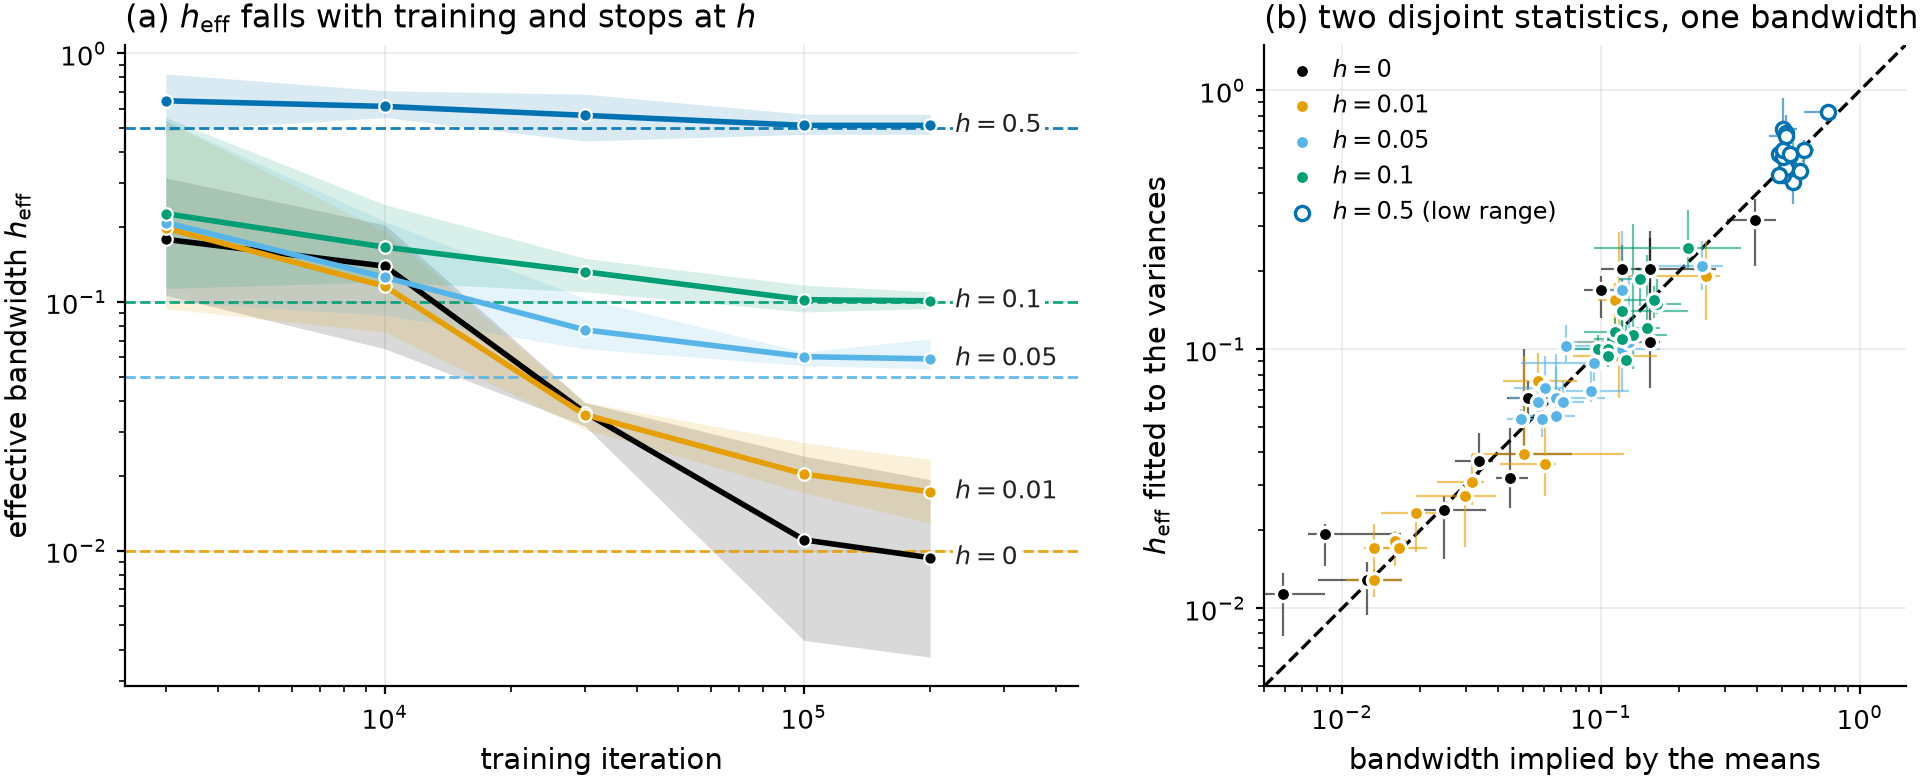
\includegraphics[width=\textwidth]{fig_heff_synthetic.png}
\caption{Linear-Gaussian problem, three seeds per bandwidth. (a) $h_{\mathrm{eff}}$
falls with training and stops just above the training bandwidth $h$ (dashed); line:
geometric mean over seeds, band: range. Checkpoints before 3000 iterations, where no
bandwidth fits, are omitted. (b) The bandwidth fitted to the variances against the one
implied by the means, with 95\% bootstrap intervals: two disjoint statistics give one
bandwidth. Open markers ($h=0.5$): the reference barely varies and
$h_{\mathrm{eff}}$ is poorly identified.}
\label{fig:heffsyn}
\end{figure}

\paragraph{CIFAR-10.} Six runs of the published setup ($h\in\{4,5\}$, three instances
each) were re-trained with weights kept at 2k--60k and analysed at $M{=}128$, 48
conditions (Figure~\ref{fig:heffcifar}). The re-runs reproduce the published ones:
$h_{\mathrm{eff}}=4.79$ and $5.81$ at 60k for seed 0, against $4.80$ and $5.75$.
From 5k iterations on, the two bandwidths agree within their intervals at 31/36
checkpoints; four of the five misses are at $h=5$ at 5k--10k, where
$h_{\mathrm{eff}}$ is still $7$--$10$, and one is at 20k.
$h_{\mathrm{eff}}$ falls monotonically in 5/6 runs and ends at $1.13$--$1.34h$; in four
runs it is still falling at 60k and in two it has levelled off, so whether it has a
floor above $h$ is open. The tracking slope rises as $h_{\mathrm{eff}}/h$ approaches
$1$ in 5/6 runs, reaching $0.66$ at $h_{\mathrm{eff}}=1.13h$. At image scale
$h_{\mathrm{eff}}$ is not a better fit to the per-condition variances than the power
law: from 30k on the two are comparable (median $R^2$ better for $h_{\mathrm{eff}}$ in
3/6 runs), and before 20k it is mostly worse.

\begin{figure}[t]
\centering
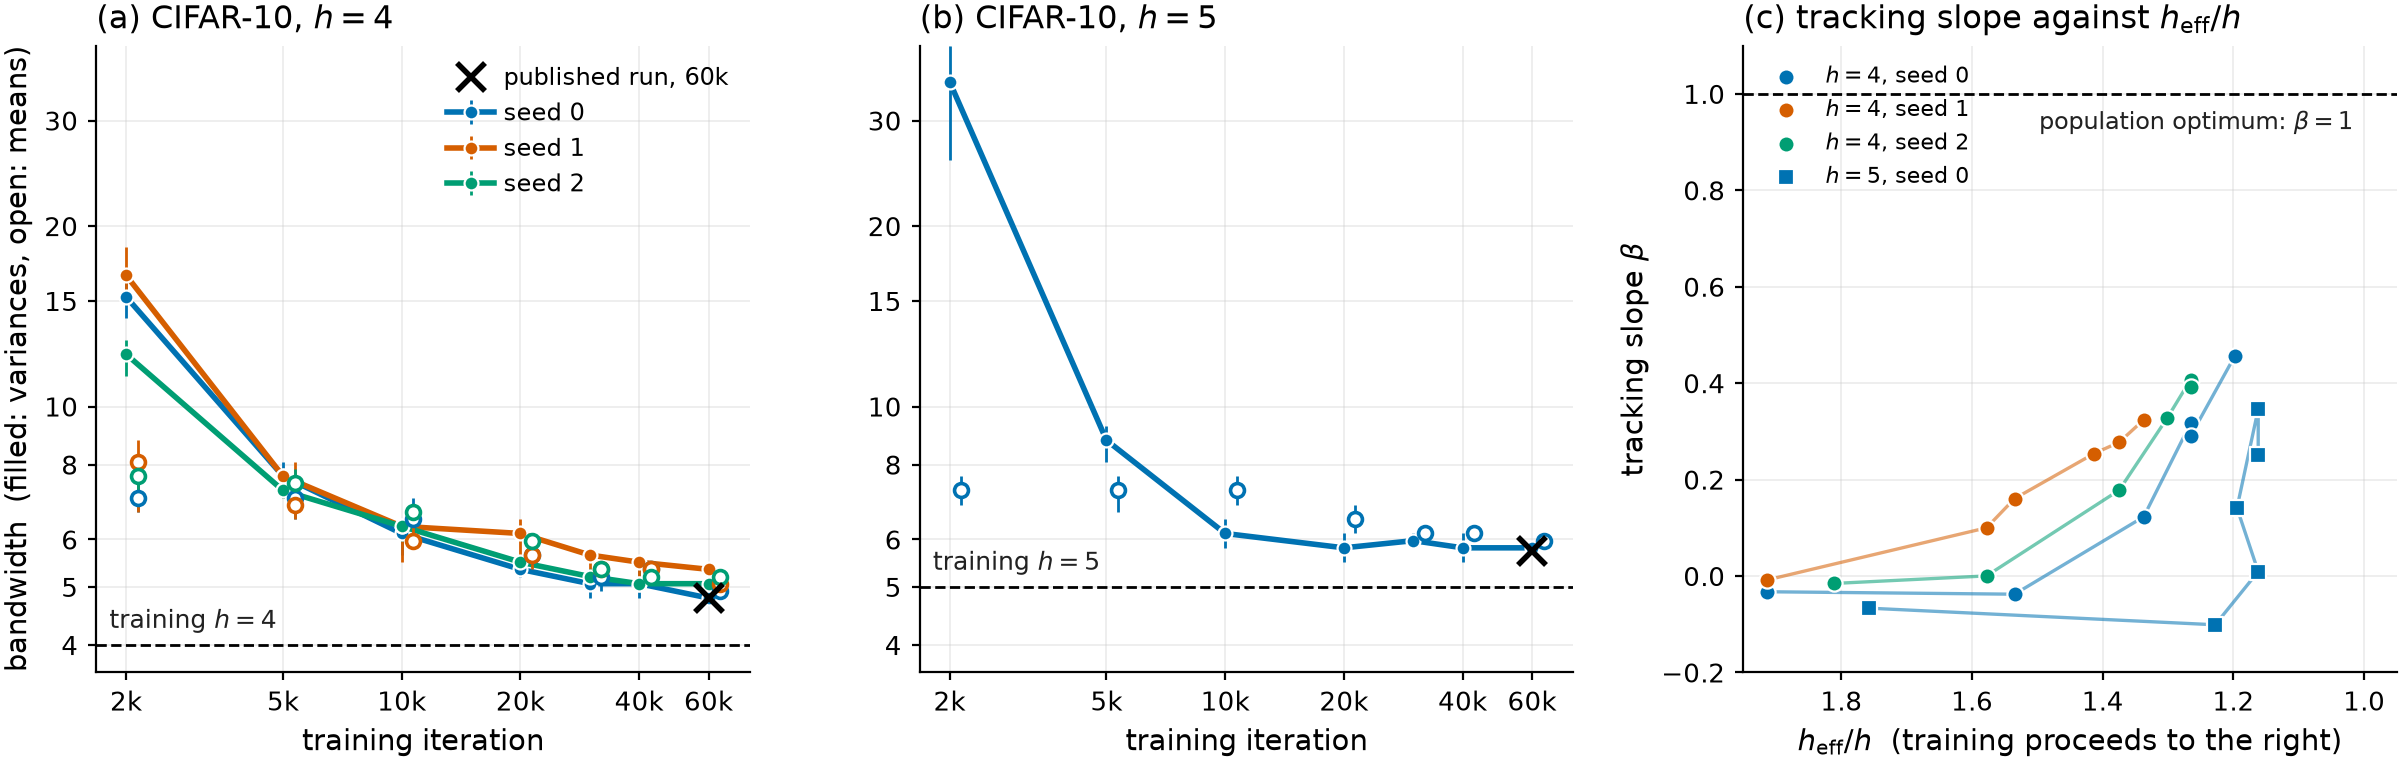
\includegraphics[width=\textwidth]{fig_heff_cifar.png}
\caption{CIFAR-10, DDPM U-Net, three instances per bandwidth. (a, b) $h_{\mathrm{eff}}$
from the variances (filled) and the bandwidth implied by the means (open), with 95\%
intervals, against training iteration; dashed: training $h$; cross: the published run
at 60k. From 5k on the two agree and fall towards $h$ without reaching it. (c) The
tracking slope $\beta$ against $h_{\mathrm{eff}}/h$; training proceeds to the right.}
\label{fig:heffcifar}
\end{figure}

% ==========================================================================
\section{Limitations and conclusion}

The exact results describe the population minimiser; the effective bandwidth is an
empirical description of trained models, supported by the agreement of two disjoint
statistics but without a theory of how $h_{\mathrm{eff}}$ depends on training time,
capacity or $N$. It is identified only where the reference varies across conditions,
and at image scale it fits the variances no better than a two-parameter power law.
Whether $h_{\mathrm{eff}}$ reaches $h$ or stops above it is open; it needs runs well
beyond $6\times10^4$ iterations. Our image experiments use one mask and
$N{=}2000$, and labels without a natural kernel, such as text, are outside scope.

Within that scope: conditional collapse is the zero-bandwidth limit of a
kernel-weighted empirical flow, label smoothing moves along that limit without leaving
the training atoms, and a trained network travels the same family of laws at a
bandwidth that training shrinks. That makes the memorisation of a conditional sampler
one number that can be read off a checkpoint.

\subsection*{Reproducibility statement}
All numbers are produced by code in the supplementary material (anonymized); the
settings above are complete for the reported runs, and full proofs are in
Appendix~\ref{app:proofs}.

\subsection*{AI use statement}
A generative-AI assistant was used to draft and edit text, to expand proofs from a
theory memorandum into their full form, to write the training and analysis code, and to
run and analyse several experiments. Every reported number is produced by the released
code from actual runs. The authors checked all proofs and verified all results against
the raw outputs, and take full responsibility for the content.

\bibliographystyle{plainnat}
\bibliography{refs}

% ==========================================================================
\appendix
\section{Proofs}
\label{app:proofs}

Throughout, conditionally on $I=i$ and for $t<1$ the map $X_0\mapsto X_t$ is an affine
bijection, so $p(x\mid I=i,t)=(1-t)^{-d}\pi_0\big(\tfrac{x-tx^i}{1-t}\big)>0$, and the
factor $(1-t)^{-d}$ cancels in every posterior over $I$. Every field below has the form
$\sum_iw_i(x,t)(x^i-x)/(1-t)$ with smooth weights in $[0,1]$ summing to one; it is
therefore locally Lipschitz on $\R^d\times[0,1)$ with $|v|\le(|x|+\max_i|x^i|)/(1-t)$,
so by Gr\"onwall each trajectory exists on $[0,1)$ and the push-forward of $\pi_0$ is the
unique solution of the continuity equation there \citep[Ch.~8]{ambrosio2008gradient}.

\paragraph{Projection.} For $m=\E[U\mid X_t,t,\widetilde Y]$,
$L_h(v)=\E|U-m|^2+\E|v-m|^2$, since the cross term vanishes by the tower property; so
$\vstar=m$ a.e.\ and $\inf_vL_h=\E\Var(U\mid X_t,t,\widetilde Y)$.

\begin{proof}[Proof of Proposition~\ref{prop:collapse}]
Distinct labels give $I=i$ from $Y=y^i$, and then $X_0=(X_t-tx^i)/(1-t)$, so
$U=x^i-X_0=(x^i-X_t)/(1-t)$ is a function of the conditioning variables. Hence
$v_0^\star=(x^i-x)/(1-t)$ and $L_0(v_0^\star)=0$. Along
$\dot x_t=(x^i-x_t)/(1-t)$, $\frac{d}{dt}\frac{x_t-x^i}{1-t}=0$, so
$x_t=(1-t)x_0+tx^i\to x^i$ for every $x_0$, and $p_1=\delta_{x^i}$.
\end{proof}

\begin{proof}[Proof of Theorem~\ref{thm:endpoint}]
Given $I=i$, $X_t$ and $\widetilde Y$ are independent, so by Bayes
$\Pr(I=i\mid X_t=x,t,\widetilde Y=y)\propto\pi_0\big(\tfrac{x-tx^i}{1-t}\big)K_h(y-y^i)=:w_i$,
and $U=(x^i-x)/(1-t)$ given $I=i$, $X_t=x$; this gives the field. Now fix $y$ and
consider the coupling $J\sim p^{(h)}(y)$, $X_0\sim\pi_0$ independent, $X_1=x^J$,
$X_t=(1-t)X_0+tX_1$. Its index posterior is
$\propto p_i^{(h)}(y)\pi_0\big(\tfrac{x-tx^i}{1-t}\big)\propto w_i$, so
$\E[X_1-X_0\mid X_t=x,t]=\vstar(x,t,y)$. For $\varphi\in C_c^\infty$,
$\frac{d}{dt}\E\varphi(X_t)=\E\langle\nabla\varphi(X_t),X_1-X_0\rangle
=\E\langle\nabla\varphi(X_t),\vstar(X_t,t,y)\rangle$, so $\law(X_t)$ solves the
continuity equation of the flow from $\pi_0$ and, by uniqueness, equals the flow's
marginal. Since $X_t\to x^J$ almost surely, $p_1=\law(x^J)=\sum_ip_i^{(h)}(y)\delta_{x^i}$.
The moments follow. As $h\to0$ with a unique nearest label $i^\star$,
$K_h(y-y^i)/K_h(y-y^{i^\star})\to0$ for $i\ne i^\star$; as $h\to\infty$,
$p_i^{(h)}\to1/N$.
\end{proof}

\begin{proof}[Proof of Proposition~\ref{prop:atomicity}]
The support statement is \eqref{eq:endpoint}. For any coupling $(X,X')$ of
$p_1(\cdot\mid y)$ and $p(\cdot\mid y)$, $X\in\{x^i\}$ almost surely, so
$\E|X-X'|^2\ge\E\dist(X',\{x^i\})^2=F(y)$; take the infimum over couplings. $F$
involves only the atoms and the posterior, and is positive because the atoms are
$p(\cdot\mid y)$-null.
\end{proof}

\begin{proof}[Proof of Proposition~\ref{prop:interp}]
Given $I=i$, $r:=x-tx^i=(1-t)X_0+\gamma Z\sim\N(0,s_t^2I_d)$, so
$\E[X_0\mid r]=\frac{1-t}{s_t^2}r$ and $\E[Z\mid r]=\frac{\gamma}{s_t^2}r$. Hence
$v^\star_\sigma(x,t,y^i)=x^i+c(t)(x-tx^i)$ with
$c=\frac{-(1-t)+\gamma\dot\gamma}{s_t^2}=\frac12\frac{d}{dt}\log s_t^2$. Then
$u_t=x_t-tx^i$ solves $\dot u=c(t)u$, so $u_t=s_tx_0$ (as $s_0=1$). Finally
$s_t^2=(1-t)[(1-t)+\sigma^2t]$, so $s_1=0$ and $x_t\to x^i$.
\end{proof}

\begin{proof}[Proof of Proposition~\ref{prop:endpointnoise}]
Given $I=i$, $r:=x-tx^i=(1-t)X_0+t\rho\xi\sim\N(0,s_t^2I_d)$ with
$s_t^2=(1-t)^2+t^2\rho^2$, so the index posterior is
$\propto\varphi_{s_t}(x-tx^i)K_h(y-y^i)$ and, by Gaussian conditioning,
$\E[U\mid X_t=x,t,I=i]=x^i+\frac{t\rho^2-(1-t)}{s_t^2}(x-tx^i)$. This field is smooth
on $\R^d\times[0,1]$ since $s_1=\rho>0$. The coupling $J\sim p^{(h)}(y)$,
$X_1=x^J+\rho\xi$ has the same index posterior and conditional velocity, so, as in the
proof of Theorem~\ref{thm:endpoint}, $p_1=\law(x^J+\rho\xi)=\sum_ip_i^{(h)}\N(x^i,\rho^2I_d)$,
with mean $\bar x_h$ and covariance $\Covh+\rho^2I_d$.
\end{proof}

\end{document}
